\documentclass[10pt]{book}
\usepackage{graphicx}
\usepackage{exercise}
\usepackage{url}
\usepackage[width=5.5in,height=8.0in,
  hmarginratio=3:2,vmarginratio=1:1]{geometry}


\begin{document}
\chapter {Directed Graphs: A Case Study of Wikipedia}
\emph{By Rachel Bobbins and Noam Rubin}
\section{Directed Graphs}
Imagine that it's 2 AM during finals week, and you're scrambling to finish your research paper on \emph{topica obscura}. Your adrenaline jumps when you finally find a relevant Wikipedia article, with links to more Wikipedia articles! You start clicking away, jumping from page to page in search of facts. An hour later, you realize you're still clicking, but these are pages you've already visited. No matter which link you click, you can't seem to discover any new pages! 

If this situation has ever happened to you, then you've unknowingly (and unfortunately) stumbled upon a knot in Wikipedia. Knots are a unique property of directed graphs. To understand them, it’s necessary to have a basic understanding of directed graphs.
\section{Directed Graphs in Code}
	 	 	
The graphs we've encountered in previous chapters are all undirected graphs. In an undirected graph, a single edge between two vertices represents a symmetric relationship between the vertices. This abstraction works well to describe some real-world systems (such as acquaintance networks and transportation networks), but it is not detailed enough to describe the Internet, including Wikipedia. Relationships between websites do not have to be symmetric -- think of all the pages that Google links to. The majority of these pages do not link back to Google. 

This non-symmetry holds true for Wikipedia as well. Page A might link to page B, but page B doesn't have to include any links to page A. To fully describe the relationship between pages A and B, we need two bits of information: whether A links to B, and whether B links to A . This is the essence of a directed graph. In a directed graph, an arc $e = (A,B)$ is an \emph{edge} from A \emph{to} B. Arcs are usually referred to as directed edges.

\begin{figure}[here]
 \centering
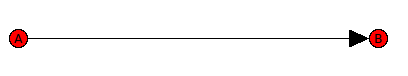
\includegraphics[scale=0.6]{../Images/DirectedGraphExample.png}
\end{figure}

As previously mentioned, knots are a unique (and sometimes cruel) property of directed graphs. A knot in a directed graph is a collection of vertices and edges with the property that every vertex in the knot has outgoing edges, and all outgoing edges from vertices in the knot terminate at other vertices in the knot. Thus it is impossible to leave the knot while following any path along its directed edges.

We mentioned the idea of knots in Wikipedia. We wondered whether such a thing was even possible. Given that there are 3,811,000+ articles on Wikipedia and they all link to different pages, it seemed unlikely that there would be a knot, but we decided to investigate.

Before writing an algorithm to determine the existence of knots in a directed graph, we extended \verb"Graph.py" to support directed graphs. The result is \verb"DirectedGraph.py", which you can download at \url{https://raw.github.com/nrubin/RachelAndNoamsDirectedGraphs/master/DirectedGraph.py}. We recommend reading through this file and making yourself familiar with the terminology. Note that Edges in DirectedGraph are represented by Arcs.

When we were designing \verb"DirectedGraph", we wanted to preserve the order of growth of \verb Vertex  and \verb Arc  lookups as they were in \verb Graph.  However, we needed to keep track of edges into a vertex and edges from a vertex. It made sense to keep track of these in separate dictionaries. Thus, out-arcs were stored in the\verb DirectedGraph  internal dictionary, and in-arcs were stored in an additional dictionary called \verb reverse_graph.  Having two dictionaries takes twice as much memory, but this seemed like a reasonable price to pay for maintaining the speed of lookups.

\section{Knotting Algorithm}

Now, back to knots. Our research found only distributed algorithms for detecting knots.\footnote{See \url{http://www.cs.utexas.edu/users/misra/scannedPdf.dir/KnotDetection.pdf}}. Distributed algorithms are designed to run concurrently on multiple processors. Identical but distinct chunks of the algorithm run on each processor, and report to each other the results of their computation. These kinds of algorithms are ideal for large research projects, but we needed an algorithm that would run on a single computer. To this end, we devised our own algorithm.

The algorithm relies heavily on a modified version of breadth-first-search, \verb"_bfsknots". It searches for all the vertices that can be reached from a given starting vertex, and returns these vertices as a set.  The function runs once for every vertex in the graph, building up a dictionary which maps a single vertex to the set of all vertices that are reachable from it.

\pagebreak
\begin{verbatim}
  def _bfsknots(self, s):
        # initialize the queue with the start vertex
        queue = [s]
        visited = set()
        on_first_vertex = True
        while queue:

            # get the next vertex
            v = queue.pop(0)

            # skip it if it's already marked
            if v in visited: continue

            # if we're on the first vertex, we're not actually visting
            if v != s or not on_first_vertex: visited.add(v)
            on_first_vertex = False
            
            for x in self.out_vertices(v):
                #if its out vertices have been cached, update visited
                if x in self._knot_cache.keys():
                    visited.update(self._knot_cache[x])
                    visited.add(x)
                    
                #otherwise add it to the queue
                elif x not in self._knot_cache.keys():
                    queue.append(x)

        return visited
\end{verbatim}

Let's say that $S_v$ is the set of vertices that are reachable from some vertex $v$, including itself. if $S_v$ is the same for all the vertices reachable from $v$, the graph has a knot.

The function \verb"has_knot" iterates through each vertex in a graph, and returns True if the previous condition holds for some vertex. If it checks the whole graph and does not find a knot, it returns False.
\begin{verbatim}
    def has_knot(self):
        """
        Returns true if directed graph has a knot.
        """
        self._knot_cache = {}
        #build the cache of which vertices are accessible from which
        for v in self:
            self._knot_cache[v] = self._bfsknots(v)

        #searches for knot
        for v in self:
            if self._knot_at_v(v):
                return True
        return False

\end{verbatim}

\begin{exercise}
 Determine the order of growth of \verb has\_knots  experimentally. You might want to review Chapter 3, Section 1. Below are several hints to help you out.
\begin{enumerate}
 \item Use \verb"DirectedGraph.add_random_edges" to generate a few thousand graphs of different sizes.

\item For each graph, time how long it takes to check if it has a knot.

\item Plot the time it took to check if the graph has a knot versus the number of vertices the graph has. Also plot against the number of edges the graph has.

\item What has more of an effect on the runtime \verb has_knots, vertices or edges?

\item From your figures, determine the order of growth of \verb has_knots .
\end{enumerate}

\end{exercise}

\begin{exercise}
 Find all the knots in a directed graph.
\begin{enumerate}
 \item Write a function, named \verb all_knots , that returns a list of all knots in a graph.
\item Building on your answer from the previous question, write a function named \verb entry_points that returns a list of all the vertices that serve as entry points into knots.
\end{enumerate}

\end{exercise}
\section{Parsing Wikipedia}

To find knots in Wikipedia, we selected 558 disjoint subsets of Wikipedia articles, organized by index. For example, the index of articles about neurobiology was used to define one subset, and the index of articles about Zimbabwe was used to define another subset. Combined, these subsets contained about 321,000 articles, or 10\% of Wikipedia. We only looked at subsets because we lacked the processing power to parse and analyze all of Wikipedia.\footnote{If you’re interested in the whole graph of Wikipedia, we recommend checking out research done by Stephen Dolan at Trinity College Dublin. His research is online here: \url{http://mu.netsoc.ie/wiki/}}. 

\section{The Structure of Wikipedia}
Of the 558 subgraphs we examined, 38\% contained at least one knot. This indicates that if you are reading articles listed on the same index page, there is a chance you will get stuck in a knot and start to see the same articles again. In actuality, the odds of this happening are much lower than 38\%, because articles can link to articles which don't share the same parent index. Our analysis ignored these links. For example, our analysis would have ignored a link from a neurobiology article to a Zimbabwe article, unless the Zimbabwe article was also listed in the neurobiology index. Furthermore, the 38\% does not imply that the graph of all of Wikipedia has a knot.

\begin{figure}[here]
 \centering
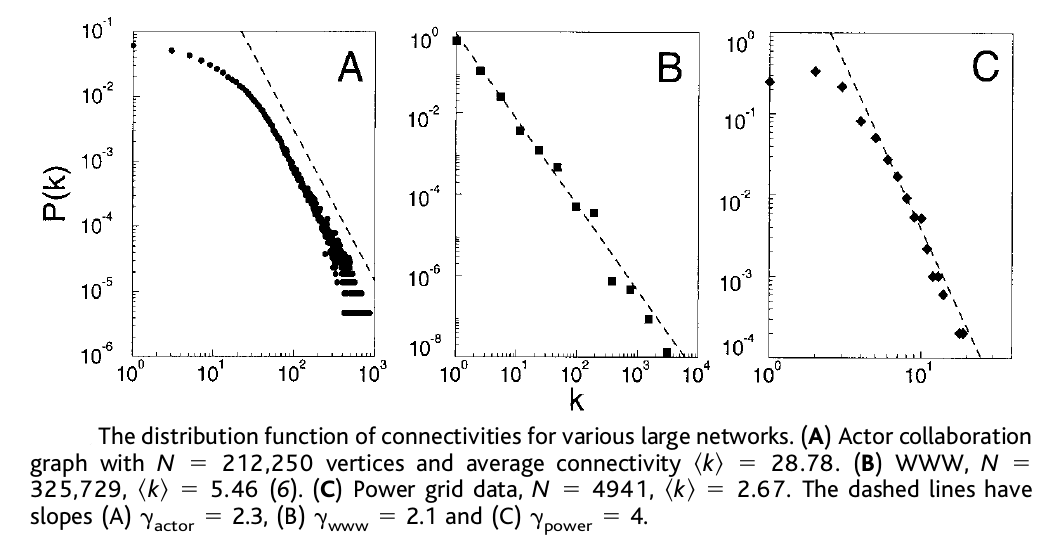
\includegraphics[scale=0.35]{../Images/BAResults.png}
\caption{The graphs from Barabasi and Albert's 1999 paper show the scale-free structure of a few undirected graphs. $k$ is the average connectivity, or degree, of the vertices in the graph, and $P(k)$ is the proportion of vertices in the graph that have this degree. Plotted on a log-log scale, scale-free networks tend to show long-tailed distributions. This is because a few vertices have the highest degree in the graph.}
\label{fig:BAGraph}
\end{figure}


Back to the original question of \emph{topica obscura}. When you started this hypothetical homework assignment, you could have chosen to use journal articles instead of Wikipedia articles. If you'd done this, you probably would have used citations to find other papers to read. You'd never have ended up in this knot. Why? Think of journal articles as vertices in a directed graph, where a directed edge represents one article citing another. Because science articles are published sequentially, and a paper cannot cite a paper that will be created in the future, this directed graph cannot have a knot. Thus, because journal articles cannot have symmetrical citations, while Wikipedia articles can, they are fundamentally different systems of organizing information.


In Barabasi and Albert's paper about scale-free networks\footnote{Barabasi, Albert-Laszlo and Albert, Reka, Emergence of Scaling in Random Networks; Science Magazine, Vol. 286, 15 October  1999.}, they analyze the underlying undirected graph of citations in scientific articles. Given that this graph must have a different structure than the graph of Wikipedia, we wondered whether the Barabasi-Albert model is applicable to Wikipedia.

\begin{figure}[here]
 \centering
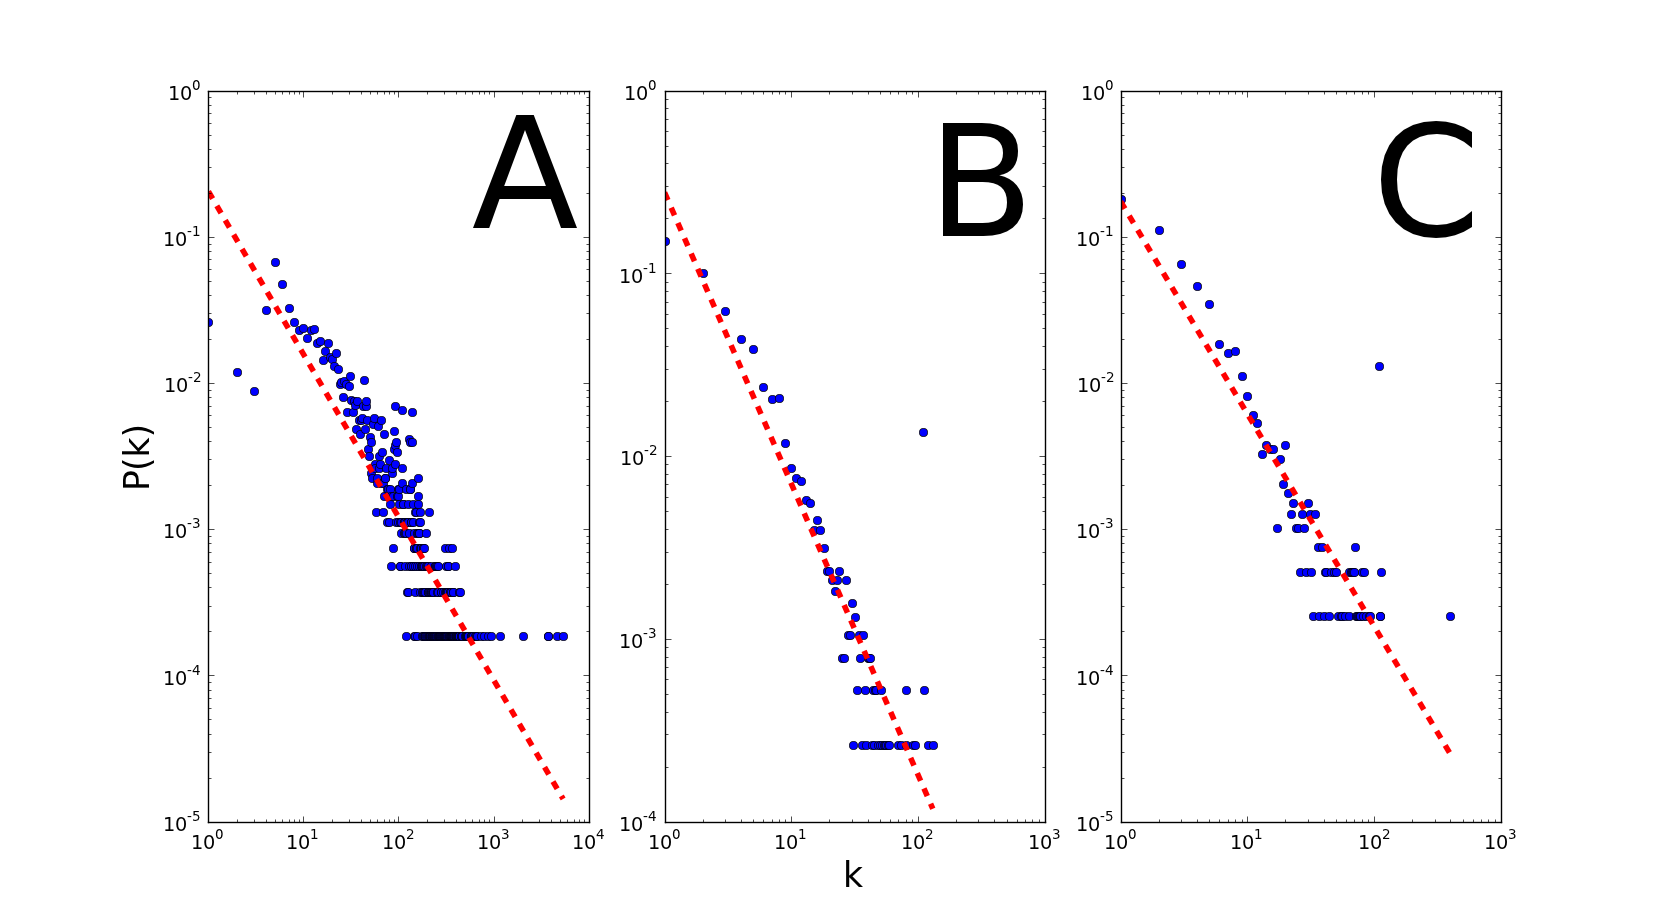
\includegraphics[scale=0.32]{../Images/WikipediaPowerLawGraph.png}
\caption{The distribution function of connectivities for various large subgraphs of Wikipedia. \textbf{(A)} Index of India-related articles with $N = 5,342$ vertices and average connectivity $ k = 53.56$.  \textbf{(B)} Index of Mathematics articles starting with C, with $N = 3813$ and average connectivity $k = 4.95$. \textbf{(C)} Index of Mathematics articles starting with S, with $N = 3950$ and average connectivity $k = 4.85$. Compared to Figure \ref{fig:BAGraph}, these three graphs also display scale-free distributions. The structure of these distinct subgraphs hints at the nature of Wikipedia as a whole, indicating that Wikipedia is possibly scale-free.}
\label{fig:PunchlineGraph}
\end{figure}

To determine the structure of the subgraphs of Wikipedia, we looked at the largest graphs and tried to recreate the results from Barabasi and Albert's 1999 paper (seen in Figure \ref{fig:BAGraph}. 

Comparing Figure \ref{fig:BAGraph} to Figure \ref{fig:PunchlineGraph}, we can see that the general structure of both is very similar. This means that the distinct subgraphs we examined are characteristically scale-free. In addition, it means that Wikipedia graphs are well-modeled by the Barabasi-Albert small world graph model.

But what does this really mean? The Barabasi-Albert model of small-world graphs is especially good at modeling preferential attachment, the phenomenon where a few of the vertices have the highest degree. The fact that both undirected graphs  and the directed graphs can have a scale-free distribution of degrees means that preferential attachment is independent of the directedness of the graph.


\begin{figure}[here]
 \centering
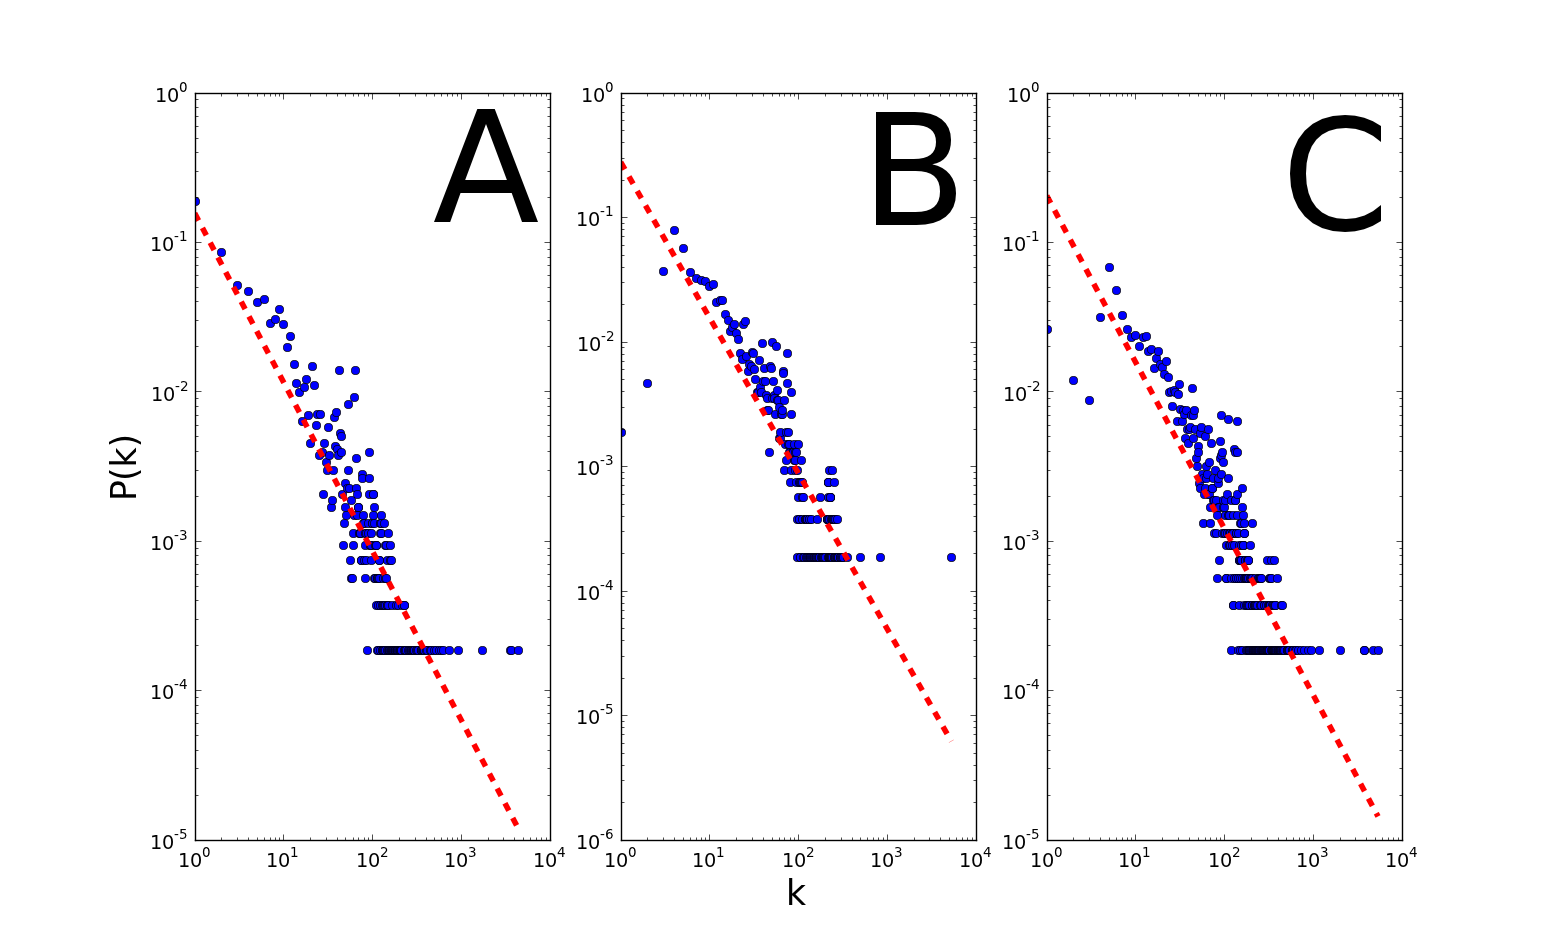
\includegraphics[scale=0.32]{../Images/AllThreeScaleFree.png}[here!]
\caption{The distribution function of connectivities for the in-degrees \textbf{(A)}, out-degrees \textbf{(B)}, and total degrees \textbf{(C)} of the vertices in the Index of India-related articles subgraph. Both the in- and out-degree distributions are scale-free, further indicating that preferential attachment is independent of directedness.}
\label{fig:AllThree}
\end{figure}


This independence is further demonstrated by Figure \ref{fig:AllThree}, which shows the degree distribution of the in, out, and total degrees of the ``Index of India-related articles''  subgraph. All three distributions are scale-free, which means that few vertices have a high in-degree and few vertices have a high out-degree. This corresponds with our findings that preferential attachment is independent of the directedness of a graph.

\pagebreak
\pagebreak

\section{Conclusion}

Since Wikipedia subgraphs display a tendency towards preferential attachment, we propose another explanation for why you keep landing on the same articles. Perhaps there is not a knot in the articles you are reading, and in fact, that set of articles is very well connected to the rest of the graph. Since subgraphs of Wikipedia are small-world, a small set of vertices will have the highest degrees in the graph. That means that if you take a random walk through the graph, the odds you'll encounter these vertices are very high. 

Barabasi and Albert's example of undirected graph of citations in science articles indicates that, even if you are traversing an undirected graph, you may encounter the same vertices over and over, without there being a knot. This small set of articles may be cited the most, so in your research for a certain topic, you're very likely to see these articles multiple times.

What does this mean for your research project? Whether you're browsing Wikipedia or JSTOR, you'll end up seeing the same highly-referenced nodes multiple times. In many ways, this can be frustrating when looking for a specific or isolated article, but it is a result of the small world nature of the graphs that represent the information you're seeking. 

\end{document}